\documentclass[11pt,a4paper]{article}

\usepackage[T1]{fontenc}
\usepackage[utf8]{inputenc}
\usepackage{lmodern}
\usepackage{microtype}
\usepackage{amsmath}
\usepackage{amssymb}
\usepackage{booktabs}
\usepackage{tabularx}
\usepackage{array}
\usepackage{enumitem}
\usepackage{pifont}
\usepackage{fancyhdr}
\usepackage{xcolor}
\usepackage{tikz}
\usepackage{pgfplots}
\usepackage[margin=2.2cm, headheight=22pt]{geometry}
\usepackage[hidelinks]{hyperref}

\usetikzlibrary{arrows.meta, positioning, calc, decorations.pathreplacing,
  shapes.geometric, fit}
\pgfplotsset{compat=1.18}

% ---------------------------------------------------------------- colors
\definecolor{accent}{RGB}{31,78,121}
\definecolor{wrongc}{RGB}{192,57,43}
\definecolor{rightc}{RGB}{30,132,73}
\definecolor{whyc}{RGB}{41,128,185}
\definecolor{stepc}{RGB}{125,60,152}
\definecolor{hookc}{RGB}{211,84,0}
\definecolor{questc}{RGB}{90,100,110}

\newcommand{\ok}{\textcolor{rightc}{\ding{51}}}
\newcommand{\bad}{\textcolor{wrongc}{\ding{55}}}

% ---------------------------------------------------------------- layout
\raggedbottom
\setlength{\parindent}{0pt}
\setlength{\parskip}{4pt}
\setlist{itemsep=2pt, topsep=3pt}
\pagestyle{fancy}
\fancyhf{}
\fancyhead[L]{\sffamily\small\color{accent}AIA \textbullet{} Exam Guide}
\fancyhead[R]{\sffamily\small\color{accent}\thepage}
\renewcommand{\headrulewidth}{0.4pt}
\renewcommand{\headrule}{\hbox to\headwidth{\color{accent!40}\leaders\hrule
  height \headrulewidth\hfill}}

% keep a heading together with at least #1 of following text
\newcommand{\keep}[1]{\par
  \ifdim\dimexpr\pagegoal-\pagetotal\relax<#1\relax\newpage\fi}

% ---------------------------------------------------------------- headings
\newcommand{\topic}[2]{%
  \keep{7cm}\bigskip
  \refstepcounter{section}%
  \addcontentsline{toc}{section}{\protect\numberline{\thesection}#1}%
  \noindent\begin{tikzpicture}
    \node[fill=accent, text=white, anchor=west, inner xsep=9pt, inner ysep=7pt, outer sep=0pt,
      text width=\linewidth-18pt, font=\sffamily\Large\bfseries]
      {\thesection\hspace{0.7em}#1\hfill{\normalsize\mdseries #2}};
  \end{tikzpicture}\par\medskip}

\newcommand{\sub}[1]{\keep{6cm}\medskip
  {\sffamily\bfseries\large\color{accent}#1}\par\smallskip}

% ---------------------------------------------------------------- callouts
\newcommand{\callout}[3]{%
  \par\smallskip\noindent
  \begin{tikzpicture}
    \node[fill=#1!7, inner xsep=10pt, inner ysep=7pt, outer sep=0pt, anchor=north west]
      (box) at (0,0) {\begin{minipage}{\dimexpr\linewidth-20pt\relax}
        {\sffamily\bfseries\small\color{#1}#2}\par\smallskip #3
      \end{minipage}};
    \fill[#1] (box.north west) rectangle ([xshift=3pt]box.south west);
  \end{tikzpicture}\par\smallskip}

\NewDocumentEnvironment{question}{+b}{\callout{questc}{Question}{#1}}{}
\NewDocumentEnvironment{yours}{+b}{\callout{wrongc}{\ding{55}\ Your answer}{#1}}{}
\NewDocumentEnvironment{correct}{+b}{\callout{rightc}{\ding{51}\ Correct answer}{#1}}{}
\NewDocumentEnvironment{why}{+b}{\callout{whyc}{Why}{#1}}{}
\NewDocumentEnvironment{steps}{+b}{\callout{stepc}{Step by step}{#1}}{}
\NewDocumentEnvironment{hook}{+b}{\callout{hookc}{Remember}{#1}}{}

% ---------------------------------------------------------------- figures
\newcommand{\fig}[2]{% body, caption
  \par\medskip\begin{center}#1\par\smallskip
  \begin{minipage}{0.9\linewidth}\centering\small\color{black!70}#2\end{minipage}
  \end{center}\medskip}

% ---------------------------------------------------------------- drawing helpers
% cuboid: #1 x, #2 y, #3 width, #4 height, #5 depth, #6 color
\newcommand{\cuboid}[6]{%
  \fill[#6!25, draw=#6!80!black] (#1,#2) -- ++(#3,0) -- ++(0,#4) -- ++(-#3,0) -- cycle;
  \fill[#6!12, draw=#6!80!black] (#1,#2+#4) -- ++(#5*0.6,#5*0.4) -- ++(#3,0) -- ++(-#5*0.6,-#5*0.4) -- cycle;
  \fill[#6!40, draw=#6!80!black] (#1+#3,#2) -- ++(#5*0.6,#5*0.4) -- ++(0,#4) -- ++(-#5*0.6,-#5*0.4) -- cycle;}
% 4x4 pooling grid with a highlighted 9: #1 x, #2 y, #3 cell column, #4 cell row
\newcommand{\poolgrid}[4]{%
  \draw[black!40] (#1,#2) grid ++(4,4);
  \draw[accent, very thick] (#1,#2) rectangle ++(4,4);
  \draw[accent, thick] (#1+2,#2) -- ++(0,4);
  \draw[accent, thick] (#1,#2+2) -- ++(4,0);
  \fill[hookc!60] (#1+#3,#2+3-#4) rectangle ++(1,1);
  \node[font=\sffamily\small\bfseries] at (#1+#3+0.5,#2+3.5-#4) {9};}

\begin{document}

% ================================================================= title
\thispagestyle{empty}
\begin{tikzpicture}[remember picture, overlay]
  \fill[accent] (current page.north west) rectangle
    ([yshift=-5.2cm]current page.north east);
  \node[anchor=west, text=white, font=\sffamily\bfseries\fontsize{30}{34}\selectfont]
    at ([xshift=2.2cm, yshift=-2.1cm]current page.north west)
    {Exam Guide};
  \node[anchor=west, text=white!85!accent, font=\sffamily\Large]
    at ([xshift=2.2cm, yshift=-3.3cm]current page.north west)
    {Automatic Image Analysis \textbullet{} learning from test-exam mistakes};
  \node[anchor=west, text=white!70!accent, font=\sffamily\normalsize]
    at ([xshift=2.2cm, yshift=-4.2cm]current page.north west)
    {Every mistake turned into a rule, a procedure, and a picture};
\end{tikzpicture}
\vspace*{4.2cm}

\sub{How to use this guide}
Each topic follows the same pattern: the \textcolor{questc}{\textbf{question}},
\textcolor{wrongc}{\textbf{what went wrong}}, the
\textcolor{rightc}{\textbf{correct answer}}, \textcolor{whyc}{\textbf{why}} it is
correct, a \textcolor{stepc}{\textbf{step-by-step}} procedure that works on any
variant of the task, and a short \textcolor{hookc}{\textbf{rule to remember}}.
Question numbers refer to \texttt{test\_exam.md}; the same task types appear in
the 2021 and 2022 exams.

\sub{Error map}
\small
\begin{tabularx}{\linewidth}{@{}l>{\raggedright\arraybackslash}X
  >{\raggedright\arraybackslash}p{2.6cm}>{\raggedright\arraybackslash}p{2.6cm}l@{}}
  \toprule
  Q & Topic & Your answer & Correct & Sec. \\
  \midrule
  2  & Classical pipeline order & wrong order & see figure & \ref{sec:pipe} \\
  10 & Backprop memory & c & a & \ref{sec:bp} \\
  11 & Backprop gate rules & a, d & a & \ref{sec:bp} \\
  12 & Bias, validation & a, b & a, b, d & \ref{sec:bias} \\
  14 & Hough point test & c, d & a & \ref{sec:hough} \\
  16 & R-table transform & b \ok & b & \ref{sec:rtable} \\
  19 & More conv filters & b, c & c, d & \ref{sec:cnn} \\
  20 & Max pooling & a, c, d & a, b, c & \ref{sec:cnn} \\
  21 & Conv parameters & 252 & 3024 & \ref{sec:cnn} \\
  23 & Histograms, entropy & 1.5 / 2 & see table & \ref{sec:sal} \\
  24 & Kadir saliency & c & b & \ref{sec:sal} \\
  27 & Backprop through time & -- & 1 & \ref{sec:bptt} \\
  29 & Poisson MLE & -- & 4.40 & \ref{sec:mle} \\
  30 & Bayes posterior & -- & 0.5027 & \ref{sec:bayes} \\
  31 & Discriminant functions & b, c & c, d & \ref{sec:disc} \\
  33 & GAN statements & last: true & last: false & \ref{sec:gan} \\
  \bottomrule
\end{tabularx}
\normalsize

% ================================================================= 1
\clearpage
\topic{General Procedure for Multiple Choice}{all questions}\label{sec:general}

Most lost points came from multi-select questions: one option too many
(Q11, Q19, Q20, Q31) or one too few (Q12). The knowledge was often there;
the checking procedure was not.

\begin{steps}
\begin{enumerate}[leftmargin=*]
  \item \textbf{Judge every option on its own.} Cover the others and ask: ``Is
        this sentence true by itself?'' Never stop after the first true option.
  \item \textbf{Look for absolute words.} ``always'', ``only'',
        ``necessarily'', ``entirely'' make a statement false in almost every case.
  \item \textbf{Check for swapped partner concepts} (figure below). The trap is a
        true sentence with one word exchanged for its partner.
  \item \textbf{Check that the option answers the question.} ``Higher
        abstraction'' is a true property of CNNs, but not an effect of \emph{more
        filters in one layer}.
  \item \textbf{Numeric answers: formula first, numbers second,} then check the
        order of magnitude.
\end{enumerate}
\end{steps}

\fig{%
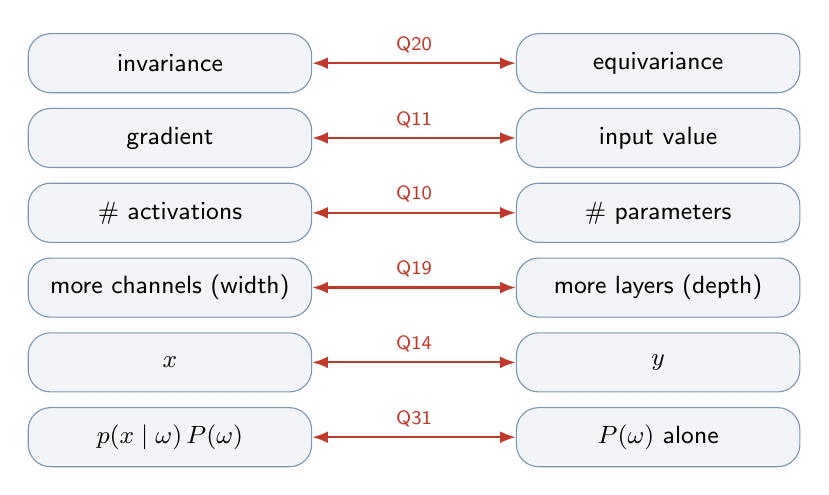
\begin{tikzpicture}[
    pill/.style={draw=accent!60, fill=accent!6, rounded corners=8pt,
      minimum width=3.6cm, minimum height=0.75cm, font=\sffamily\small},
    swap/.style={{Latex[length=2mm]}-{Latex[length=2mm]}, wrongc, thick}]
  \foreach \l/\r/\q [count=\i] in {
      invariance/equivariance/Q20,
      gradient/input value/Q11,
      \# activations/\# parameters/Q10,
      more channels (width)/more layers (depth)/Q19,
      $x$/$y$/Q14,
      $p(x\mid\omega)\,P(\omega)$/$P(\omega)$ alone/Q31} {
    \node[pill] (l\i) at (0,-0.95*\i) {\l};
    \node[pill] (r\i) at (6.2,-0.95*\i) {\r};
    \draw[swap] (l\i) -- node[above, font=\scriptsize\sffamily, text=wrongc] {\q} (r\i);
  }
\end{tikzpicture}}{Partner concepts that were swapped in the test exam. When an
option contains one of them, re-read it with the partner and decide which one
makes the sentence true.}

% ================================================================= 2
\topic{Classical Computer Vision Pipeline}{Q2}\label{sec:pipe}

\begin{question}
Bring Data Preprocessing, Feature Selection, Feature Extraction, Feature
Preprocessing, Post processing, and Classifier into the correct order.
\end{question}

\begin{correct}
Data Preprocessing $\to$ Feature Extraction $\to$ Feature Selection $\to$
Feature Preprocessing $\to$ Classifier $\to$ Post processing.
\end{correct}

\fig{%
\resizebox{\linewidth}{!}{%
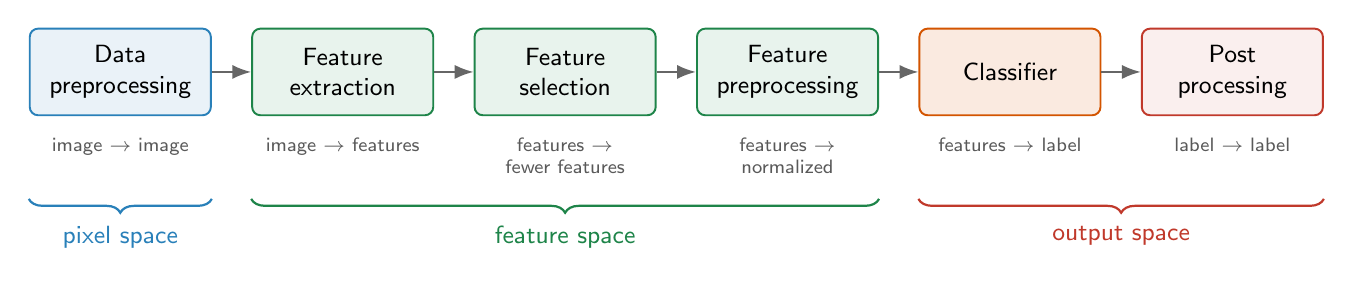
\begin{tikzpicture}[
    stage/.style={draw, rounded corners=3pt, align=center, minimum width=2.3cm,
      minimum height=1.1cm, font=\sffamily\small, line width=0.7pt},
    io/.style={font=\sffamily\scriptsize, text=black!65, align=center},
    arr/.style={-{Latex[length=2.4mm]}, thick, black!60}]
  \node[stage, fill=whyc!10, draw=whyc] (d) {Data\\preprocessing};
  \node[stage, fill=rightc!10, draw=rightc, right=0.5cm of d] (e) {Feature\\extraction};
  \node[stage, fill=rightc!10, draw=rightc, right=0.5cm of e] (s) {Feature\\selection};
  \node[stage, fill=rightc!10, draw=rightc, right=0.5cm of s] (p) {Feature\\preprocessing};
  \node[stage, fill=hookc!12, draw=hookc, right=0.5cm of p] (c) {Classifier};
  \node[stage, fill=wrongc!8, draw=wrongc, right=0.5cm of c] (o) {Post\\processing};
  \foreach \a/\b in {d/e, e/s, s/p, p/c, c/o} \draw[arr] (\a) -- (\b);
  \node[io, below=0.15cm of d] {image $\to$ image};
  \node[io, below=0.15cm of e] {image $\to$ features};
  \node[io, below=0.15cm of s] {features $\to$\\fewer features};
  \node[io, below=0.15cm of p] {features $\to$\\normalized};
  \node[io, below=0.15cm of c] {features $\to$ label};
  \node[io, below=0.15cm of o] {label $\to$ label};
  \draw[decorate, decoration={brace, amplitude=5pt, mirror}, whyc, thick]
    ([yshift=-1.05cm]d.south west) -- node[below=6pt, font=\sffamily\small] {pixel space}
    ([yshift=-1.05cm]d.south east);
  \draw[decorate, decoration={brace, amplitude=5pt, mirror}, rightc, thick]
    ([yshift=-1.05cm]e.south west) -- node[below=6pt, font=\sffamily\small] {feature space}
    ([yshift=-1.05cm]p.south east);
  \draw[decorate, decoration={brace, amplitude=5pt, mirror}, wrongc, thick]
    ([yshift=-1.05cm]c.south west) -- node[below=6pt, font=\sffamily\small] {output space}
    ([yshift=-1.05cm]o.south east);
\end{tikzpicture}}}{The six stages, sorted by what goes in and what comes out.
Everything in pixel space comes first; everything that needs labels comes last.}

\begin{steps}
\begin{enumerate}[leftmargin=*]
  \item Write down input and output type of each stage (image, features, label).
  \item Chain them so that each output type is the next input type.
  \item Inside feature space: you can only \emph{select} features that have
        been \emph{extracted}; you normalize only the features that survive the
        selection, directly before the classifier.
\end{enumerate}
\end{steps}

\begin{hook}
\textbf{D}ata $\to$ \textbf{E}xtract $\to$ \textbf{S}elect $\to$
\textbf{P}repare $\to$ \textbf{C}lassify $\to$ \textbf{P}ost.
\end{hook}

% ================================================================= 3
\topic{Backpropagation}{Q10, Q11}\label{sec:bp}

\sub{Memory consumption (Q10)}

\begin{yours}
``Memory is proportional to the number of trainable parameters.''
\end{yours}
\begin{correct}
``Memory is proportional to the combined output dimensionalities of the nodes in
the network.''
\end{correct}

\begin{why}
The backward pass needs, at every node, the value that node produced in the
forward pass: the input $x$ for the derivative of $w\cdot x$, the ReLU input to
know whether it was active. All these \textbf{activations} are stored until the
backward pass. Their number is the sum of the output sizes of all nodes (times the
batch size). Convolutional layers have few parameters but huge outputs, so
parameter count and memory are not proportional.
\end{why}

\fig{%
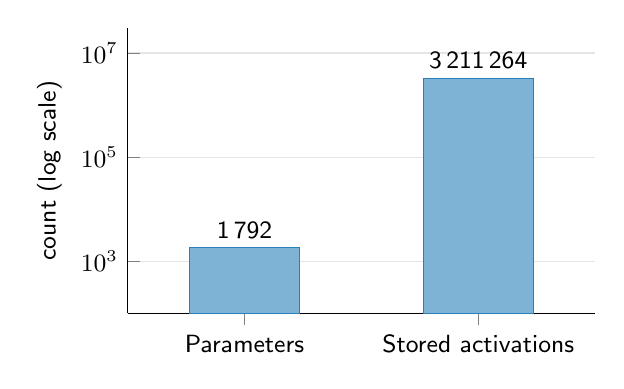
\begin{tikzpicture}
\begin{axis}[
    ybar, bar width=1.4cm, width=0.62\linewidth, height=5.2cm,
    ymode=log, ymin=100, ymax=3e7, log origin=infty,
    symbolic x coords={Parameters, Stored activations},
    xtick=data, enlarge x limits=0.5,
    ylabel={count (log scale)},
    tick label style={font=\sffamily\small},
    label style={font=\sffamily\small},
    nodes near coords, every node near coord/.append style={font=\sffamily\small},
    point meta=explicit symbolic, axis lines*=left, ymajorgrids,
    grid style={black!10}]
  \addplot[fill=whyc!60, draw=whyc] coordinates
    {(Parameters,1792) [1\,792] (Stored activations,3211264) [3\,211\,264]};
\end{axis}
\end{tikzpicture}}{One $3\times3$ convolution, $3\to64$ channels, on a
$224\times224$ image: under two thousand parameters, but over three million
output values that must be kept for the backward pass (per image).}

Also: one update step needs exactly \textbf{one} forward and \textbf{one}
backward pass. Options with ``multiple passes'' are false.

\sub{Gate rules (Q11)}

\begin{yours}
Ticked ``Addition nodes backpropagate their inputs''.
\end{yours}
\begin{correct}
Only ``Backpropagation allows for efficient optimization of computational graphs
with gradient descent''.
\end{correct}

\fig{%
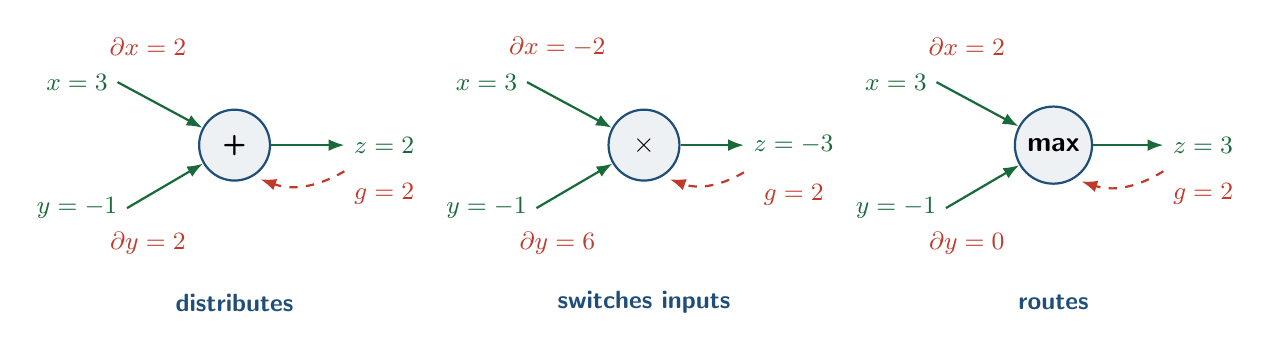
\begin{tikzpicture}[
    gate/.style={circle, draw=accent, fill=accent!8, thick, minimum size=0.9cm,
      font=\sffamily\bfseries},
    fwd/.style={-{Latex[length=2mm]}, rightc!80!black, thick},
    bwd/.style={-{Latex[length=2mm]}, wrongc, thick, dashed},
    val/.style={font=\sffamily\small, text=rightc!80!black},
    grd/.style={font=\sffamily\small, text=wrongc}]
  \foreach \op/\name/\z/\gx/\gy/\rl [count=\i] in {
      +/add/2/2/2/{distributes},
      $\times$/mul/-3/-2/6/{switches inputs},
      max/max/3/2/0/{routes}} {
    \begin{scope}[xshift=(\i-1)*5.2cm]
      \node[gate] (g) at (0,0) {\op};
      \node[val] (x) at (-2,0.8) {$x=3$};
      \node[val] (y) at (-2,-0.8) {$y=-1$};
      \node[val] (z) at (1.9,0) {$z=\z$};
      \draw[fwd] (x.east) -- (g);
      \draw[fwd] (y.east) -- (g);
      \draw[fwd] (g) -- (z);
      \draw[bwd] ([yshift=-3pt]z.south west) to[bend left=25] ([yshift=-3pt]g.south east);
      \node[grd, anchor=north] at ([yshift=-4pt]z.south) {$g=2$};
      \node[grd] at (-1.1,1.25) {$\partial x = \gx$};
      \node[grd] at (-1.1,-1.25) {$\partial y = \gy$};
      \node[font=\sffamily\small\bfseries, text=accent] at (0,-2) {\rl};
    \end{scope}}
\end{tikzpicture}}{Forward values (green) and backward gradients (red) for the
same inputs $x=3$, $y=-1$ and upstream gradient $g=2$. Only the multiplication
node uses the input values, and it swaps them: $\partial x = g\cdot y$,
$\partial y = g\cdot x$.}

\begin{center}\small
\begin{tabular}{@{}lll@{}}
  \toprule
  Node & Forward & Backward (upstream gradient $g$) \\
  \midrule
  Addition $z=x+y$ & sum & $\partial x = g$, $\partial y = g$ \quad (copy the gradient) \\
  Multiplication $z=xy$ & product & $\partial x = g\,y$, $\partial y = g\,x$ \quad (swap the inputs) \\
  Max $z=\max(x,y)$ & maximum & $g$ to the larger input, $0$ to the other \\
  \bottomrule
\end{tabular}
\end{center}

\begin{why}
The addition node passes on the \emph{gradient}, never its inputs.
Backpropagation also does \emph{not} reduce SGD noise (that comes from
mini-batches) and does \emph{not} guarantee the optimum (the loss is non-convex).
It only computes the exact gradient efficiently.
\end{why}

% ================================================================= 4
\topic{Bias, Variance, and Model Complexity}{Q12}\label{sec:bias}

\begin{yours}
a, b \quad(missed d: ``A model with high bias tends to underfit the data.'')
\end{yours}

\fig{%
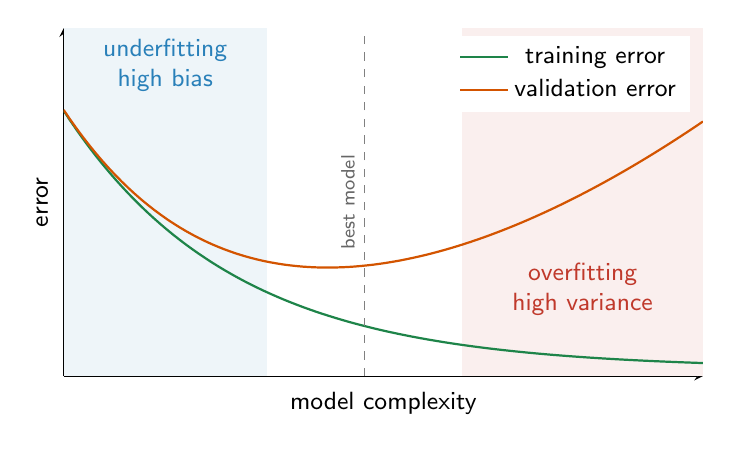
\begin{tikzpicture}
\begin{axis}[
    width=0.8\linewidth, height=6cm, domain=0.5:9, samples=100,
    xlabel={model complexity}, ylabel={error}, ymin=0, ymax=1.4,
    xtick=\empty, ytick=\empty, axis lines=left,
    label style={font=\sffamily\small},
    legend style={font=\sffamily\small, draw=none, at={(0.98,0.98)}, anchor=north east}]
  \fill[whyc!8] (axis cs:0.5,0) rectangle (axis cs:3.2,1.4);
  \fill[wrongc!8] (axis cs:5.8,0) rectangle (axis cs:9,1.4);
  \addplot[thick, rightc] {1.3*exp(-0.45*x)+0.03};
  \addplot[thick, hookc] {1.3*exp(-0.45*x)+0.03+0.012*x^2};
  \legend{training error, validation error}
  \node[font=\sffamily\small, text=whyc, align=center] at (axis cs:1.85,1.25)
    {underfitting\\high bias};
  \node[font=\sffamily\small, text=wrongc, align=center] at (axis cs:7.4,0.35)
    {overfitting\\high variance};
  \draw[dashed, black!50] (axis cs:4.5,0) -- (axis cs:4.5,1.4);
  \node[font=\sffamily\scriptsize, text=black!60, rotate=90, anchor=south]
    at (axis cs:4.5,0.7) {best model};
\end{axis}
\end{tikzpicture}}{Training error always falls with complexity. Validation error
falls, then rises again. High bias sits on the left (both errors high), high
variance on the right (small training, large validation error).}

\begin{center}\small
\begin{tabularx}{\linewidth}{@{}Xcp{6.3cm}@{}}
  \toprule
  Statement & True? & Reason \\
  \midrule
  Small training error $\Rightarrow$ sufficient complexity & \ok & the model is
    flexible enough to fit the data \\
  Small validation error $\Rightarrow$ good performance & \ok & unseen data
    estimates generalization \\
  Small training error $\Rightarrow$ good performance & \bad & the model could
    overfit (right side of the plot) \\
  High bias $\Rightarrow$ underfitting & \ok & too simple, it misses even the
    training data (left side) \\
  \bottomrule
\end{tabularx}
\end{center}

\begin{hook}
\textbf{B}ias $=$ \textbf{B}elow the data (underfit). \quad
\textbf{V}ariance $=$ \textbf{V}olatile, fits the noise (overfit).
\end{hook}

% ================================================================= 5
\topic{Hough Transform: Point on a Line}{Q14}\label{sec:hough}

\begin{question}
Which lines $(\theta,\rho)$ pass through $(x,y)=(2,10)$? \
Options: $(0,2)$, $(0.75\pi,-10)$, $(0,10)$, $(0.5\pi,2)$.
\end{question}
\begin{yours}
$(0,10)$ and $(0.5\pi,2)$ \quad --- the roles of $x$ and $y$ were swapped.
\end{yours}
\begin{correct}
Only $(\theta,\rho)=(0,2)$.
\end{correct}

\fig{%
\begin{minipage}{0.47\linewidth}\centering
\begin{tikzpicture}
\begin{axis}[
    width=0.95\linewidth, height=6.2cm,
    xmin=-2, xmax=16, ymin=-3, ymax=13, axis lines=left,
    xlabel={$x$}, ylabel={$y$}, xtick={0,2,10}, ytick={0,2,10},
    tick label style={font=\scriptsize}, label style={font=\small},
    title={\sffamily\small image space},
    legend style={font=\scriptsize, draw=none, at={(0.5,-0.22)}, anchor=north},
    legend columns=2, legend cell align=left]
  \addplot[very thick, rightc] coordinates {(2,-3) (2,13)};
  \addplot[thick, wrongc, dashed] coordinates {(10,-3) (10,13)};
  \addplot[thick, stepc, dashed] coordinates {(-2,2) (16,2)};
  \addplot[thick, hookc, dashed, domain=11.142:16] {x-14.142};
  \legend{{$(0,2)$: $x=2$}, {$(0,10)$: $x=10$}, {$(\frac{\pi}{2},2)$: $y=2$},
    {$(\frac{3\pi}{4},-10)$}}
  \addplot[only marks, mark=*, mark size=2.8pt, accent, forget plot] coordinates {(2,10)};
  \node[font=\scriptsize, text=accent, anchor=west] at (axis cs:2.4,10) {$(2,10)$};
\end{axis}
\end{tikzpicture}
\end{minipage}\hfill
\begin{minipage}{0.5\linewidth}\centering
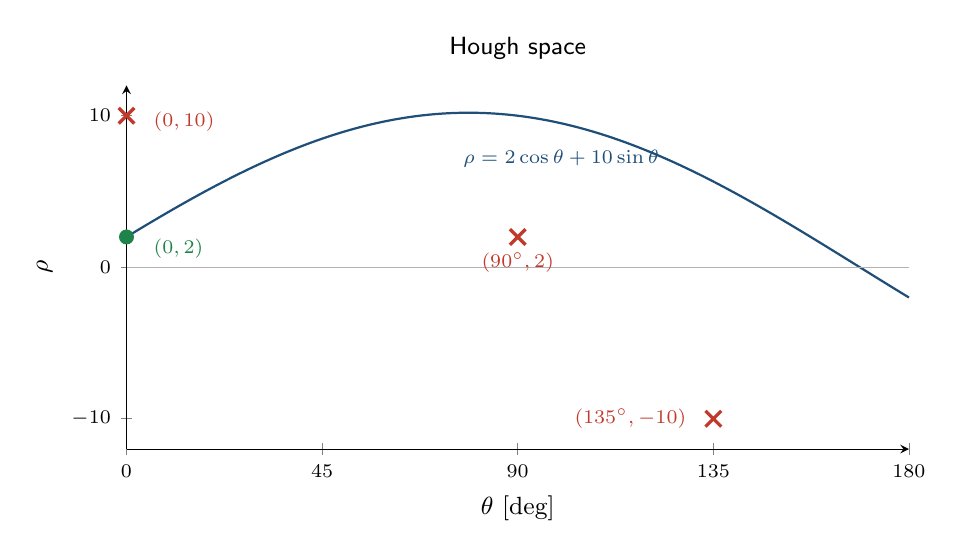
\begin{tikzpicture}
\begin{axis}[
    width=0.95\linewidth, height=6.2cm, clip=false,
    xmin=0, xmax=180, ymin=-12, ymax=12, domain=0:180, samples=120,
    xlabel={$\theta$ [deg]}, ylabel={$\rho$}, xtick={0,45,90,135,180},
    axis lines=left, tick label style={font=\scriptsize},
    label style={font=\small}, title={\sffamily\small Hough space}]
  \addplot[thick, accent] {2*cos(x)+10*sin(x)};
  \addplot[only marks, mark=*, mark size=2.5pt, rightc] coordinates {(0,2)};
  \addplot[only marks, mark=x, mark size=4pt, very thick, wrongc]
    coordinates {(0,10) (90,2) (135,-10)};
  \draw[black!30] (axis cs:0,0) -- (axis cs:180,0);
  \node[font=\scriptsize\sffamily, text=accent, anchor=north] at (axis cs:100,8.4) {$\rho = 2\cos\theta + 10\sin\theta$};
  \node[font=\scriptsize\sffamily, text=rightc, anchor=west] at (axis cs:4,1.2) {$(0,2)$};
  \node[font=\scriptsize\sffamily, text=wrongc, anchor=west] at (axis cs:4,9.6) {$(0,10)$};
  \node[font=\scriptsize\sffamily, text=wrongc, anchor=north] at (axis cs:90,1.6) {$(90^\circ,2)$};
  \node[font=\scriptsize\sffamily, text=wrongc, anchor=east] at (axis cs:131,-10) {$(135^\circ,-10)$};
\end{axis}
\end{tikzpicture}
\end{minipage}}{Left: the four candidate lines; only $x=2$ passes through the
point. Right: in Hough space the point becomes a sinusoid; a line passes through
the point exactly when its $(\theta,\rho)$ lies on the curve.}

\begin{steps}
\begin{enumerate}[leftmargin=*]
  \item Write the line equation: $\boxed{\rho = x\cos\theta + y\sin\theta}$.
  \item Insert the point: $\rho(\theta) = 2\cos\theta + 10\sin\theta$.
  \item Evaluate every option and compare with the given $\rho$:
\end{enumerate}
\centering\small
\begin{tabular}{@{}cccccc@{}}
  \toprule
  Option & $\cos\theta$ & $\sin\theta$ & $2\cos\theta+10\sin\theta$ & given $\rho$ & \\
  \midrule
  $(0,2)$ & $1$ & $0$ & $2$ & $2$ & \ok \\
  $(0.75\pi,-10)$ & $-0.707$ & $0.707$ & $5.66$ & $-10$ & \bad \\
  $(0,10)$ & $1$ & $0$ & $2$ & $10$ & \bad \\
  $(0.5\pi,2)$ & $0$ & $1$ & $10$ & $2$ & \bad \\
  \bottomrule
\end{tabular}
\end{steps}

\begin{hook}
$\theta=0$: $\rho = x$, the line is \textbf{vertical} ($x=\rho$). \quad
$\theta=\pi/2$: $\rho = y$, the line is \textbf{horizontal} ($y=\rho$).
Always compute; never match numbers by eye.
\end{hook}

% ================================================================= 6
\topic{Generalized Hough Transform: R-Table}{Q16}\label{sec:rtable}

Answered correctly (b). The reasoning below keeps it reproducible for other
scales, angles, and table ranges.

\begin{question}
Transform the R-table with scale $s=2$ and a counter-clockwise rotation of
$\varphi=180^\circ$. Rows: $[0,45)$: $(1,2);(3,4)$ \quad $[45,90)$: -- \quad
$[90,135)$: $(5,6);(7,8)$ \quad $[135,180)$: $(9,10)$.
\end{question}

\fig{%
\begin{minipage}{0.48\linewidth}\centering
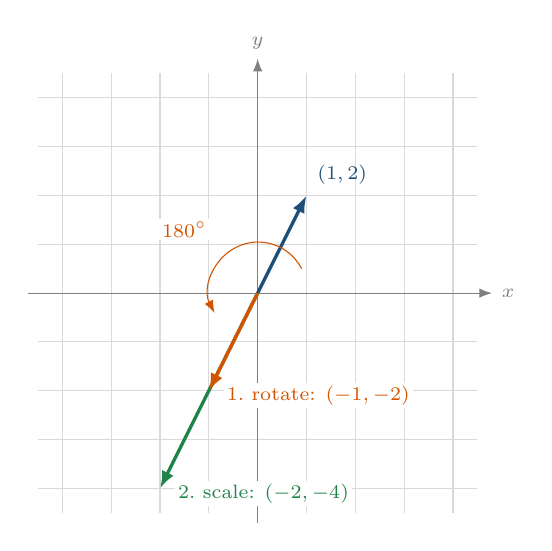
\begin{tikzpicture}[scale=0.62,
    vec/.style={-{Latex[length=2.2mm]}, very thick}]
  \draw[black!15] (-4.5,-4.5) grid (4.5,4.5);
  \draw[-{Latex[length=1.6mm]}, black!50] (-4.7,0) -- (4.8,0) node[right, font=\scriptsize] {$x$};
  \draw[-{Latex[length=1.6mm]}, black!50] (0,-4.7) -- (0,4.8) node[above, font=\scriptsize] {$y$};
  \draw[vec, accent] (0,0) -- (1,2) node[above right, font=\scriptsize] {$(1,2)$};
  \draw[vec, rightc] (0,0) -- (-2,-4);
  \draw[vec, hookc] (0,0) -- (-1,-2);
  \node[font=\scriptsize, text=hookc, anchor=west, fill=white, inner sep=1pt] at (-0.7,-2.1) {1.~rotate: $(-1,-2)$};
  \node[font=\scriptsize, text=rightc, anchor=west, fill=white, inner sep=1pt] at (-1.7,-4.1) {2.~scale: $(-2,-4)$};
  \draw[hookc, -{Latex[length=1.6mm]}] (0.9,0.5) arc (27:207:1) ;
  \node[font=\scriptsize, text=hookc, fill=white, inner sep=1pt] at (-1.5,1.3) {$180^\circ$};
\end{tikzpicture}\par\small displacement vectors
\end{minipage}\hfill
\begin{minipage}{0.48\linewidth}\centering
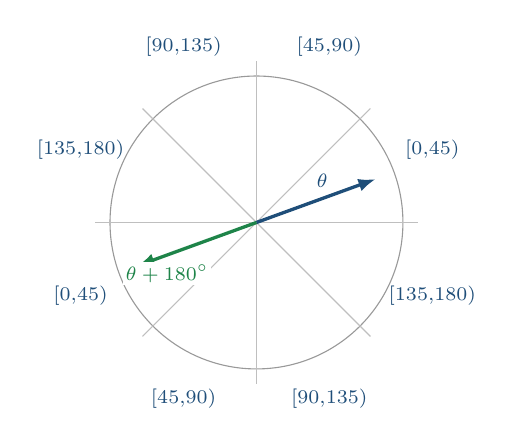
\begin{tikzpicture}[scale=0.62]
  \draw[black!40] (0,0) circle (3);
  \foreach \a in {0,45,90,135} {
    \draw[black!25] (0,0) -- (\a:3.3);
    \draw[black!25] (0,0) -- (\a+180:3.3);
  }
  \foreach \a/\l in {22.5/{[0,45)}, 67.5/{[45,90)}, 112.5/{[90,135)}, 157.5/{[135,180)}} {
    \node[font=\scriptsize, text=accent] at (\a:3.9) {\l};
    \node[font=\scriptsize, text=accent] at (\a+180:3.9) {\l};
  }
  \draw[-{Latex[length=2.2mm]}, very thick, accent] (0,0) -- (20:2.6) node[pos=0.55, above, font=\scriptsize] {$\theta$};
  \draw[-{Latex[length=2.2mm]}, very thick, rightc] (0,0) -- (200:2.6) node[pos=0.75, below=2pt, font=\scriptsize, fill=white, inner sep=1pt] {$\theta+180^\circ$};
\end{tikzpicture}\par\small gradient orientation modulo $180^\circ$
\end{minipage}}{Left: rotating by $180^\circ$ negates each displacement, scaling
by $2$ doubles it. Right: a gradient direction rotated by $180^\circ$ lies on the
same line, so with a table over $[0^\circ,180^\circ)$ it stays in its row.}

\begin{steps}
\begin{enumerate}[leftmargin=*]
  \item \textbf{Scale}: multiply every displacement by $s$. Rows stay, since
        scaling does not change gradient directions.
  \item \textbf{Rotate the vectors} by $\varphi$. For $180^\circ$:
        $(d_x,d_y)\mapsto(-d_x,-d_y)$.
  \item \textbf{Rotate the rows}: every entry moves to the row for $\theta+\varphi$.
        Check the table range! Over $[0^\circ,180^\circ)$, orientations are taken
        modulo $180^\circ$, so $\theta+180^\circ\equiv\theta$: nothing moves.
  \item Result: $(1,2)\to(-2,-4)$, $(3,4)\to(-6,-8)$, $(5,6)\to(-10,-12)$,
        $(7,8)\to(-14,-16)$, $(9,10)\to(-18,-20)$; rows unchanged. $\Rightarrow$ \textbf{b}.
\end{enumerate}
\end{steps}

\begin{hook}
Distractors: only shifted rows (a), swapped components $=$ reflection (c),
unchanged (d). If the table covers $[0^\circ,360^\circ)$, a $180^\circ$ rotation
\emph{does} move rows. Translation never changes an R-table.
\end{hook}

% ================================================================= 7
\topic{CNN Layers}{Q19, Q20, Q21}\label{sec:cnn}

\sub{Number of weights (Q21)}

\begin{yours}
$252 = 3\cdot3\cdot28$ \quad --- the input channels were forgotten.
\end{yours}
\begin{correct}
$3\cdot3\cdot12\cdot28 = 3024$
\end{correct}

\fig{%
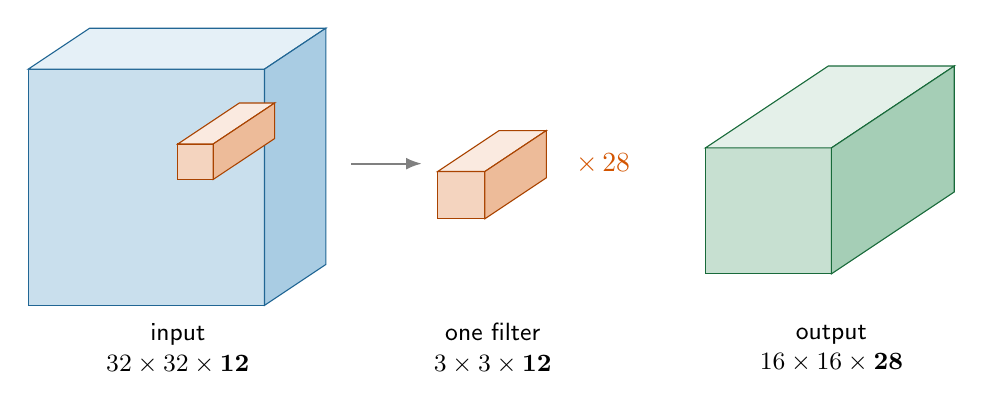
\begin{tikzpicture}[x={(1cm,0)}, y={(0,1cm)}]
  \cuboid{0}{0}{3}{3}{1.3}{whyc}
  \node[font=\sffamily\small, align=center] at (1.9,-0.55) {input\\$32\times32\times\mathbf{12}$};
  \cuboid{1.9}{1.6}{0.45}{0.45}{1.3}{hookc}
  \cuboid{5.2}{1.1}{0.6}{0.6}{1.3}{hookc}
  \node[font=\sffamily\small, align=center] at (5.9,-0.55) {one filter\\$3\times3\times\mathbf{12}$};
  \node[font=\sffamily\bfseries, text=hookc] at (7.3,1.8) {$\times\,28$};
  \cuboid{8.6}{0.4}{1.6}{1.6}{2.6}{rightc}
  \node[font=\sffamily\small, align=center] at (10.2,-0.55) {output\\$16\times16\times\mathbf{28}$};
  \draw[-{Latex[length=2mm]}, thick, black!50] (4.1,1.8) -- (5.0,1.8);
\end{tikzpicture}}{Every filter spans the \emph{full input depth}
($3\times3\times12 = 108$ weights). One filter produces one output channel, so
$28$ filters are needed. The spatial sizes ($32\to16$) do not enter the count;
they only reveal the stride.}

\begin{steps}
\[
\#\text{weights} = K_h\cdot K_w\cdot C_\text{in}\cdot C_\text{out}
 = 3\cdot3\cdot12\cdot28 = 3024,
\qquad \#\text{biases} = C_\text{out} = 28 .
\]
Stride (Q22): $W_\text{out} = \left\lfloor \frac{W_\text{in}+2P-K}{S}\right\rfloor + 1$.
Halving the size ($148\to74$ with $K=3$, $P=1$) means $S=2$.
\end{steps}

\sub{More filters in one layer (Q19)}

\begin{yours}
Ticked ``Higher abstraction capabilities of the layer''.
\end{yours}
\begin{correct}
Increase in output dimensionality; increased number of features the layer can
respond to.
\end{correct}

\begin{center}\small
\begin{tabular}{@{}lll@{}}
  \toprule
  Change & What it adds & Abstraction? \\
  \midrule
  More filters (\textbf{width}) & more output channels $=$ more feature detectors
    at the same level & \bad \\
  More layers (\textbf{depth}) & larger receptive field, features of features & \ok \\
  \bottomrule
\end{tabular}
\end{center}

\sub{Effects of max pooling (Q20)}

\begin{yours}
Ticked ``Translation equivariance'' instead of ``Translation invariance''.
\end{yours}
\begin{correct}
Dimensionality reduction, translation invariance, loss of spatial/relational
information.
\end{correct}

\fig{%
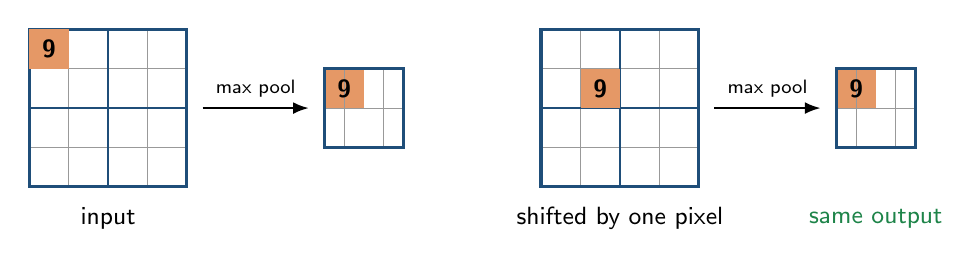
\begin{tikzpicture}[scale=0.5]
  \poolgrid{0}{0}{0}{0}
  \node[font=\sffamily\small] at (2,-0.8) {input};
  \draw[-{Latex[length=2mm]}, thick] (4.4,2) -- node[above, font=\sffamily\scriptsize] {max pool} (7.1,2);
  \draw[black!40] (7.5,1) grid ++(2,2);
  \fill[hookc!60] (7.5,2) rectangle ++(1,1);
  \draw[black!40] (7.5,1) grid ++(2,2);
  \draw[accent, very thick] (7.5,1) rectangle ++(2,2);
  \node[font=\sffamily\small\bfseries] at (8,2.5) {9};
  \poolgrid{13}{0}{1}{1}
  \node[font=\sffamily\small] at (15,-0.8) {shifted by one pixel};
  \draw[-{Latex[length=2mm]}, thick] (17.4,2) -- node[above, font=\sffamily\scriptsize] {max pool} (20.1,2);
  \draw[black!40] (20.5,1) grid ++(2,2);
  \fill[hookc!60] (20.5,2) rectangle ++(1,1);
  \draw[black!40] (20.5,1) grid ++(2,2);
  \draw[accent, very thick] (20.5,1) rectangle ++(2,2);
  \node[font=\sffamily\small\bfseries] at (21,2.5) {9};
  \node[font=\sffamily\small, text=rightc] at (21.5,-0.8) {same output};
\end{tikzpicture}}{A small shift inside a $2\times2$ pooling block does not change
the pooled output: \textbf{invariance}. The price is that the exact position is
lost. An \emph{equivariant} operation (convolution) would shift its output along
with the input.}

\begin{hook}
\textbf{Conv $=$ Equivariant} (output moves with the input). \quad
\textbf{Pool $=$ Invariant} (output stays).
\end{hook}

% ================================================================= 8
\topic{Histograms, Entropy, and Saliency}{Q23, Q24}\label{sec:sal}

\sub{Matching histograms and entropy values (Q23)}

The task had 8 drag-and-drop placements (4 histograms, then 4 entropy values),
each worth $0.25$ points. A score of $1.5/2$ means two wrong placements, typically
\textbf{one swapped pair}.

\fig{%
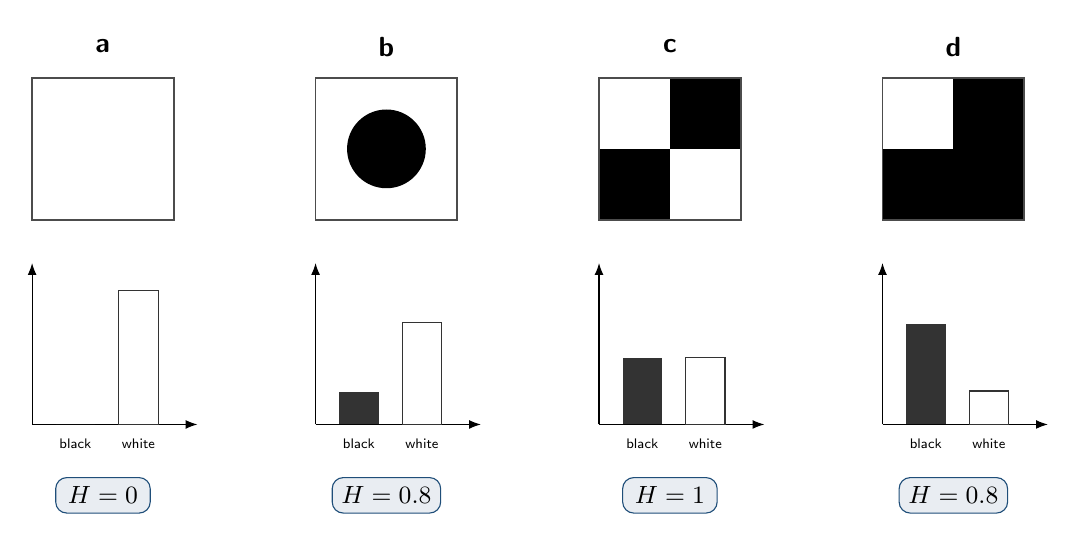
\begin{tikzpicture}[
    patch/.style={draw=black!70, line width=0.6pt},
    lbl/.style={font=\sffamily\bfseries}]
  \foreach \n/\pb/\pw/\H [count=\i] in {a/0/1/0, b/0.24/0.76/0.8, c/0.5/0.5/1, d/0.75/0.25/0.8} {
    \begin{scope}[xshift=(\i-1)*3.6cm]
      \node[lbl] at (0.9,2.2) {\n};
      % histogram
      \draw[-{Latex[length=1.5mm]}] (0,-2.6) -- (2.1,-2.6);
      \draw[-{Latex[length=1.5mm]}] (0,-2.6) -- (0,-0.55);
      \fill[black!80] (0.3,-2.6) rectangle ++(0.5,1.7*\pb);
      \draw[black!80, fill=white] (1.1,-2.6) rectangle ++(0.5,1.7*\pw);
      \node[font=\sffamily\tiny] at (0.55,-2.85) {black};
      \node[font=\sffamily\tiny] at (1.35,-2.85) {white};
      % entropy badge
      \node[draw=accent, fill=accent!10, rounded corners=4pt, font=\sffamily\small,
        minimum width=1.2cm] at (0.9,-3.5) {$H=\H$};
    \end{scope}}
  % patches
  \draw[patch, fill=white] (0,0) rectangle (1.8,1.8);
  \begin{scope}[xshift=3.6cm]
    \draw[patch, fill=white] (0,0) rectangle (1.8,1.8);
    \fill[black] (0.9,0.9) circle (0.5);
  \end{scope}
  \begin{scope}[xshift=7.2cm]
    \fill[black] (0.9,0.9) rectangle (1.8,1.8);
    \fill[black] (0,0) rectangle (0.9,0.9);
    \draw[patch] (0,0) rectangle (1.8,1.8);
  \end{scope}
  \begin{scope}[xshift=10.8cm]
    \fill[black] (0.9,0) rectangle (1.8,1.8);
    \fill[black] (0,0) rectangle (0.9,0.9);
    \draw[patch] (0,0) rectangle (1.8,1.8);
  \end{scope}
\end{tikzpicture}}{Correct matching. The histogram counts only \emph{how many}
black and white pixels there are, never \emph{where} they are. Patches b and d
have mirrored histograms but the same entropy.}

\begin{steps}
\begin{enumerate}[leftmargin=*]
  \item \textbf{Fix the axis orientation first.} The single-bar histogram must
        belong to the all-white patch a. Its bar sits on the right, so the axis
        runs from black (left) to white (right).
  \item For each patch, estimate the black/white fraction and pick the
        histogram with those bar heights. Mostly white (b): tall bar right.
        Mostly black (d): tall bar left.
  \item Compute $H = -\sum_i p_i\log_2 p_i$: one value $\Rightarrow 0$; $50/50
        \Rightarrow 1$; $25/75 \Rightarrow 0.81$.
  \item The two ``$0.8$'' tokens look identical but may be graded as distinct
        items. Place each next to the histogram it belongs to.
\end{enumerate}
\end{steps}

\fig{%
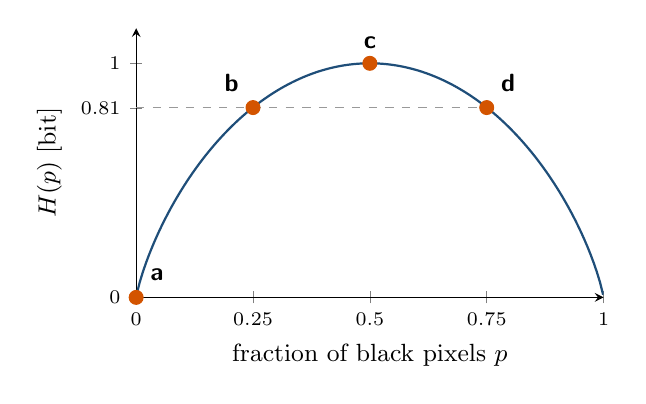
\begin{tikzpicture}
\begin{axis}[
    width=0.62\linewidth, height=5cm, domain=0.001:0.999, samples=150,
    xlabel={fraction of black pixels $p$}, ylabel={$H(p)$ [bit]},
    xmin=0, xmax=1, ymin=0, ymax=1.15, axis lines=left,
    xtick={0,0.25,0.5,0.75,1}, ytick={0,0.81,1},
    tick label style={font=\scriptsize}, label style={font=\small}]
  \addplot[thick, accent] {-(x*ln(x)+(1-x)*ln(1-x))/ln(2)};
  \addplot[only marks, mark=*, mark size=2.5pt, hookc]
    coordinates {(0,0) (0.25,0.811) (0.5,1) (0.75,0.811)};
  \node[font=\sffamily\small\bfseries, anchor=south west] at (axis cs:0.01,0.03) {a};
  \node[font=\sffamily\small\bfseries, anchor=south east] at (axis cs:0.24,0.84) {b};
  \node[font=\sffamily\small\bfseries, anchor=south] at (axis cs:0.5,1.02) {c};
  \node[font=\sffamily\small\bfseries, anchor=south west] at (axis cs:0.76,0.84) {d};
  \draw[dashed, black!40] (axis cs:0,0.811) -- (axis cs:0.75,0.811);
\end{axis}
\end{tikzpicture}}{Binary entropy is symmetric: $25\,\%$ black and $75\,\%$ black
give the same $0.81$ bit.}

\sub{Most salient patch after Kadir et al.\ (Q24)}

\begin{yours}
c (the patch with the highest entropy).
\end{yours}
\begin{correct}
b (the black disk).
\end{correct}

\begin{why}
Kadir--Brady saliency is \textbf{not} entropy alone:
\[
y(s_p,x) = H_D(s_p,x)\cdot W_D(s_p,x),
\qquad
W_D(s,x) = s\!\int\Big|\tfrac{\partial}{\partial s}p(I,s,x)\Big|\,\mathrm{d}I .
\]
$H_D$ is taken at a scale $s_p$ where the entropy has a \textbf{peak} over scale,
and $W_D$ is large only if the histogram \textbf{changes across scale}. A patch
whose statistics look the same at every window size scores zero, however high
its entropy.
\end{why}

\fig{%
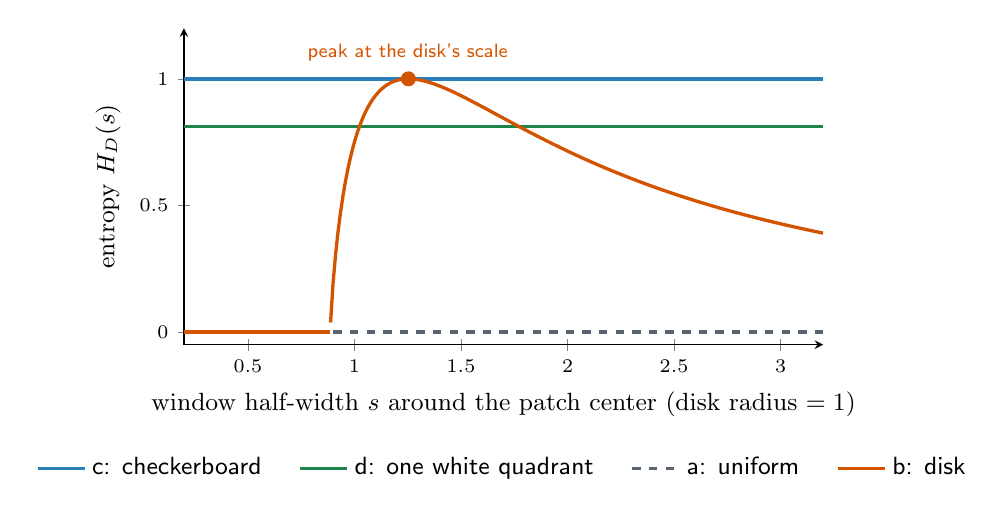
\begin{tikzpicture}
\begin{axis}[
    width=0.8\linewidth, height=5.6cm, xmin=0.2, xmax=3.2, ymin=-0.05, ymax=1.2,
    xlabel={window half-width $s$ around the patch center (disk radius $=1$)},
    ylabel={entropy $H_D(s)$}, axis lines=left,
    tick label style={font=\scriptsize}, label style={font=\small},
    legend style={font=\sffamily\small, draw=none, at={(0.5,-0.32)}, anchor=north},
    legend columns=4, legend cell align=left,
    legend style={/tikz/every even column/.append style={column sep=0.4cm}}]
  \addplot[very thick, whyc, domain=0.2:3.2] {1.0};
  \addplot[very thick, rightc, domain=0.2:3.2] {0.811};
  \addplot[very thick, questc, dashed, domain=0.2:3.2] {0};
  \addplot[very thick, hookc, domain=0.2:0.886] {0};
  \addplot[very thick, hookc, domain=0.888:3.2, samples=200, forget plot]
    {-( (pi/(4*x^2))*ln(pi/(4*x^2)) + (1-pi/(4*x^2))*ln(1-pi/(4*x^2)) )/ln(2)};
  \legend{c: checkerboard, d: one white quadrant, a: uniform, b: disk}
  \addplot[only marks, mark=*, mark size=2.5pt, hookc, forget plot] coordinates {(1.2533,1)};
  \node[font=\sffamily\scriptsize, text=hookc, anchor=south] at (axis cs:1.25,1.03) {peak at the disk's scale};
\end{axis}
\end{tikzpicture}}{Entropy as a function of window size, window centered on each
patch. Checkerboard, quadrant, and uniform patch keep the same black/white ratio
at every size: flat curves, no peak, $W_D = 0$. Only the disk shows a peak where
the window just encloses it; there the histogram changes fastest.}

\begin{steps}
\begin{enumerate}[leftmargin=*]
  \item Grow a window around the center of each patch and imagine its histogram.
  \item Does the histogram change with window size? If not, the entropy curve is
        flat: no peak, not salient (a, c, d).
  \item Is there a window size where the entropy is maximal and then falls again?
        That is a \emph{characteristic scale}: salient (b).
\end{enumerate}
\end{steps}

\begin{hook}
Kadir saliency favors \textbf{isolated blobs with a characteristic scale}, not
the maximum-entropy patch. Entropy alone is insufficient because the intensity
distribution contains \textbf{no spatial information} (Q25).
\end{hook}

% ================================================================= 9
\topic{Backpropagation Through Time}{Q27}\label{sec:bptt}

\begin{question}
RNN cell $h_t = a\,h_{t-1} + a\,x_t$ with $a=1$, $h_0=0$, sequence
$(x_1,x_2,x_3)=(1,4,5)$. What is the derivative with respect to $x_1$?
\end{question}
\begin{correct}
$\partial h_3/\partial x_1 = a^3 = 1$
\end{correct}

\fig{%
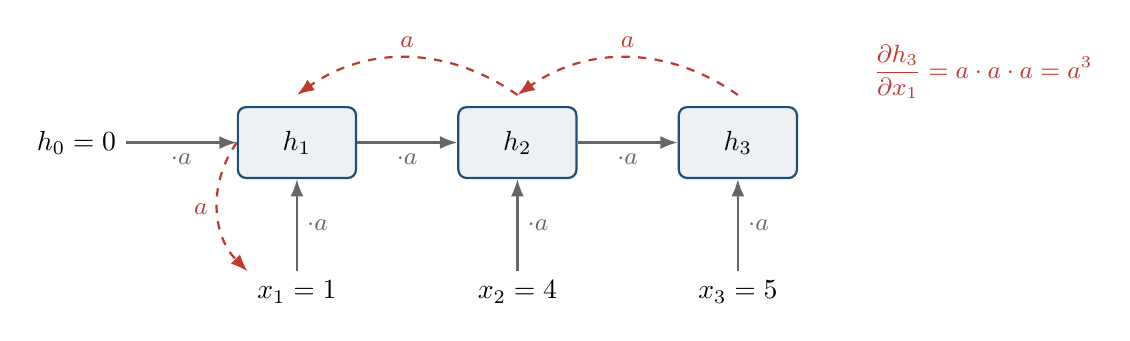
\begin{tikzpicture}[
    cell/.style={draw=accent, fill=accent!8, rounded corners=3pt, thick,
      minimum width=1.5cm, minimum height=0.9cm, font=\sffamily},
    inp/.style={font=\sffamily},
    fwd/.style={-{Latex[length=2.2mm]}, thick, black!60},
    bwd/.style={-{Latex[length=2.2mm]}, thick, wrongc, dashed}]
  \node[inp] (h0) at (0,0) {$h_0=0$};
  \node[cell] (h1) at (2.8,0) {$h_1$};
  \node[cell] (h2) at (5.6,0) {$h_2$};
  \node[cell] (h3) at (8.4,0) {$h_3$};
  \node[inp] (x1) at (2.8,-1.9) {$x_1=1$};
  \node[inp] (x2) at (5.6,-1.9) {$x_2=4$};
  \node[inp] (x3) at (8.4,-1.9) {$x_3=5$};
  \draw[fwd] (h0) -- node[below, font=\small] {$\cdot a$} (h1);
  \draw[fwd] (h1) -- node[below, font=\small] {$\cdot a$} (h2);
  \draw[fwd] (h2) -- node[below, font=\small] {$\cdot a$} (h3);
  \foreach \i in {1,2,3} \draw[fwd] (x\i) -- node[right, font=\small] {$\cdot a$} (h\i);
  \draw[bwd] ([yshift=4pt]h3.north) to[bend right=35] node[above, font=\small] {$a$} ([yshift=4pt]h2.north);
  \draw[bwd] ([yshift=4pt]h2.north) to[bend right=35] node[above, font=\small] {$a$} ([yshift=4pt]h1.north);
  \draw[bwd] (h1.west) to[bend right=40] node[left, font=\small] {$a$} (x1.north west);
  \node[font=\sffamily\small, text=wrongc, anchor=west] at (10,0.9) {$\dfrac{\partial h_3}{\partial x_1} = a\cdot a\cdot a = a^3$};
\end{tikzpicture}}{Unrolled over three time steps with shared weight $a$. The
gradient travels backwards (red) and picks up one factor $a$ per step.}

\begin{steps}
\begin{enumerate}[leftmargin=*]
  \item \textbf{Unroll}: $h_1 = a x_1$, \quad $h_2 = a^2 x_1 + a x_2$, \quad
        $h_3 = a^3 x_1 + a^2 x_2 + a x_3$.
  \item \textbf{Chain rule backwards through time}:
        $\frac{\partial h_3}{\partial x_1} =
         \frac{\partial h_3}{\partial h_2}\cdot\frac{\partial h_2}{\partial h_1}\cdot
         \frac{\partial h_1}{\partial x_1} = a^3$.
  \item \textbf{Insert} $a=1$: result $1$. The values $x_2=4$, $x_3=5$ are
        distractors, because the cell is linear.
\end{enumerate}
\end{steps}

\fig{%
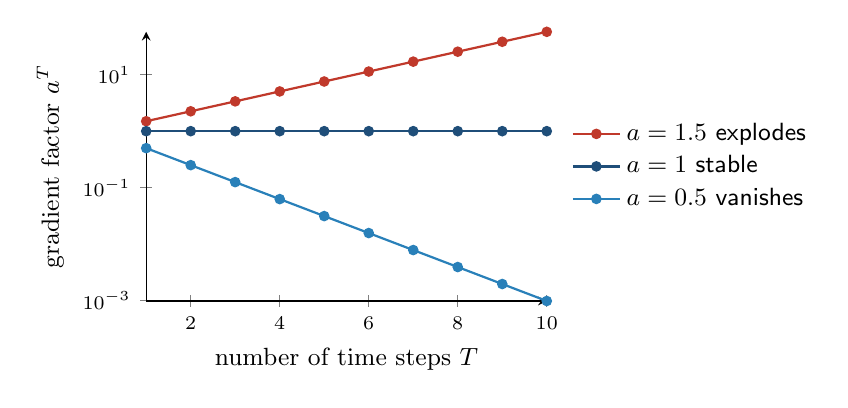
\begin{tikzpicture}
\begin{axis}[
    width=0.55\linewidth, height=5cm, ymode=log, xmin=1, xmax=10,
    xlabel={number of time steps $T$}, ylabel={gradient factor $a^T$},
    axis lines=left, samples at={1,...,10},
    tick label style={font=\scriptsize}, label style={font=\small},
    legend style={font=\sffamily\small, draw=none, at={(1.04,0.5)}, anchor=west},
    legend cell align=left]
  \addplot[thick, wrongc, mark=*, mark size=1.5pt] {1.5^x};
  \addplot[thick, accent, mark=*, mark size=1.5pt] {1^x};
  \addplot[thick, whyc, mark=*, mark size=1.5pt] {0.5^x};
  \legend{$a=1.5$ explodes, $a=1$ stable, $a=0.5$ vanishes}
\end{axis}
\end{tikzpicture}}{The same product $a^T$ explains the vanishing and exploding
gradient problem of RNNs.}

% ================================================================= 10
\topic{Maximum Likelihood Estimation}{Q29}\label{sec:mle}

\begin{question}
Error counts $X=\{2,8,4,2,6\}$, model $P(k)=\lambda^k e^{-\lambda}/k!$.
Find $\lambda_\text{MLE}$.
\end{question}
\begin{correct}
$\lambda_\text{MLE} = \bar{k} = 22/5 = 4.40$
\end{correct}

\begin{steps}
\begin{enumerate}[leftmargin=*]
  \item Likelihood (product over samples):
        $L(\lambda) = \prod_i \lambda^{k_i}e^{-\lambda}/k_i!$
  \item Log-likelihood: $\ell(\lambda) = \big(\sum_i k_i\big)\ln\lambda - n\lambda
        - \sum_i\ln k_i!$
  \item Derivative $=0$: $\frac{\sum_i k_i}{\lambda} - n = 0$
        $\;\Rightarrow\; \lambda_\text{MLE} = \frac1n\sum_i k_i$
  \item Insert: $(2+8+4+2+6)/5 = 22/5 = 4.40$
\end{enumerate}
\end{steps}

\fig{%
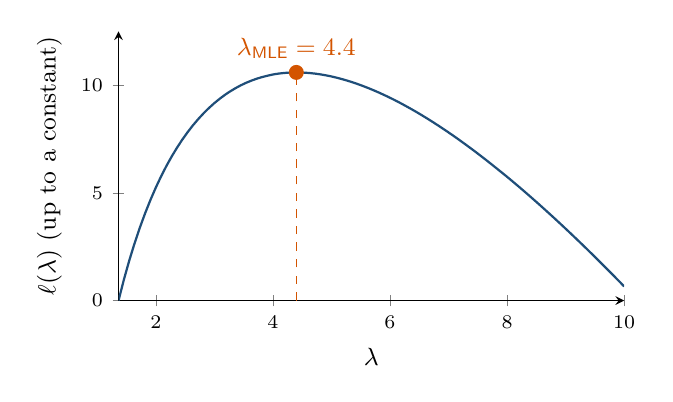
\begin{tikzpicture}
\begin{axis}[
    width=0.66\linewidth, height=5cm, domain=1:10, samples=100,
    xlabel={$\lambda$}, ylabel={$\ell(\lambda)$ (up to a constant)},
    axis lines=left, ymin=0, ymax=12.5,
    tick label style={font=\scriptsize}, label style={font=\small}]
  \addplot[thick, accent] {22*ln(x)-5*x};
  \draw[dashed, hookc] (axis cs:4.4,0) -- (axis cs:4.4,10.6);
  \addplot[only marks, mark=*, mark size=2.5pt, hookc] coordinates {(4.4,10.595)};
  \node[font=\sffamily\small, text=hookc, anchor=south] at (axis cs:4.4,10.8)
    {$\lambda_\text{MLE}=4.4$};
\end{axis}
\end{tikzpicture}}{The log-likelihood $22\ln\lambda - 5\lambda$ peaks at the
sample mean.}

\begin{center}\small
\begin{tabular}{@{}ll@{}}
  \toprule
  Distribution & MLE \\
  \midrule
  Poisson $\lambda$ & sample mean \\
  Bernoulli $p$ & fraction of ones \\
  Gaussian $\mu$ & sample mean \\
  Gaussian $\sigma^2$ & $\frac1n\sum_i(x_i-\hat\mu)^2$ (divide by $n$, not $n-1$) \\
  Exponential $\lambda$ & $1/$sample mean \\
  \bottomrule
\end{tabular}
\end{center}

% ================================================================= 11
\topic{Bayesian Posterior}{Q30}\label{sec:bayes}

\begin{question}
$P(D\mid\Omega_1)=0.52$, $P(D\mid\Omega_2)=0.58$, $P(\Omega_1)=0.53$,
$P(\Omega_2)=0.47$. Find $P(\Omega_1\mid D)$ to four decimals.
\end{question}
\begin{correct}
$0.5027$
\end{correct}

\fig{%
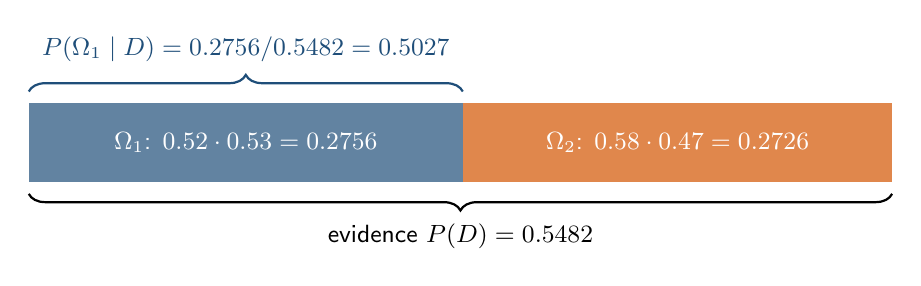
\begin{tikzpicture}[x=20cm]
  \fill[accent!70] (0,0) rectangle (0.2756,1);
  \fill[hookc!70] (0.2756,0) rectangle (0.5482,1);
  \node[text=white, font=\sffamily\small, align=center] at (0.1378,0.5)
    {$\Omega_1$: $0.52\cdot0.53 = 0.2756$};
  \node[text=white, font=\sffamily\small, align=center] at (0.4119,0.5)
    {$\Omega_2$: $0.58\cdot0.47 = 0.2726$};
  \draw[decorate, decoration={brace, amplitude=6pt, mirror}, thick]
    (0,-0.15) -- node[below=7pt, font=\sffamily\small]
    {evidence $P(D) = 0.5482$} (0.5482,-0.15);
  \draw[decorate, decoration={brace, amplitude=6pt}, thick, accent]
    (0,1.15) -- node[above=7pt, font=\sffamily\small, text=accent]
    {$P(\Omega_1\mid D) = 0.2756/0.5482 = 0.5027$} (0.2756,1.15);
\end{tikzpicture}}{Each bar is likelihood $\times$ prior. The posterior is one
bar's share of the total. $\Omega_2$ has the higher likelihood, but its lower prior
makes $\Omega_1$ slightly more probable.}

\begin{steps}
\begin{enumerate}[leftmargin=*]
  \item Numerator per hypothesis: likelihood $\times$ prior.
  \item Evidence: sum of \emph{all} numerators.
  \item Posterior: own numerator $/$ evidence. Check that all posteriors sum to 1
        ($0.5027 + 0.4973$).
  \item Keep four or more decimals in between; round only at the end.
\end{enumerate}
\end{steps}

% ================================================================= 12
\topic{Discriminant Functions}{Q31}\label{sec:disc}

\begin{yours}
$P(\omega_i)$ and $\sqrt{p(x\mid\omega_i)P(\omega_i)}$ \quad --- missed
$P(\omega_i\mid x)$.
\end{yours}
\begin{correct}
$\sqrt{p(x\mid\omega_i)P(\omega_i)}$ and $P(\omega_i\mid x)$.
\end{correct}

\begin{why}
$g_i(x)$ is a valid discriminant function if it \textbf{ranks the classes like
the posterior} $P(\omega_i\mid x)$ for \textbf{every} $x$. The posterior itself
qualifies trivially, and so does any strictly increasing transform applied equally
to all classes. $P(\omega_i)$ ignores $x$: it picks the same class for every input.
\end{why}

\fig{%
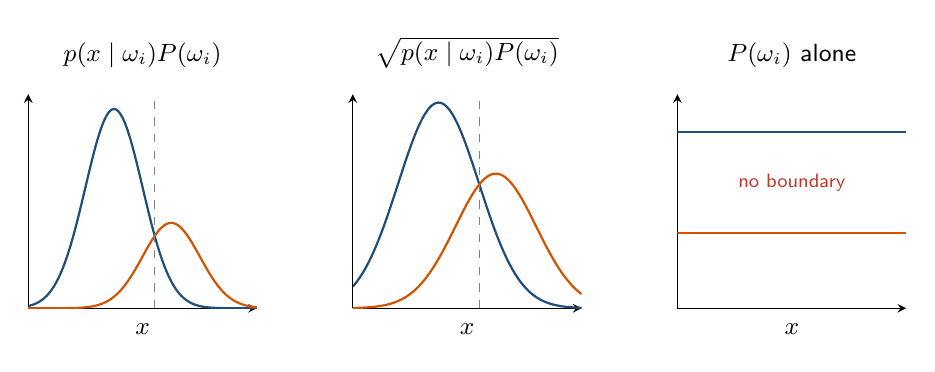
\begin{tikzpicture}
\pgfplotsset{small panel/.style={
    width=0.37\linewidth, height=4.3cm, domain=-3:5, samples=100,
    xlabel={$x$}, axis lines=left, xtick=\empty, ytick=\empty,
    label style={font=\small}, title style={font=\sffamily\small}}}
\begin{axis}[small panel, title={$p(x\mid\omega_i)P(\omega_i)$}, ymin=0, ymax=0.3]
  \addplot[thick, accent] {0.7*exp(-x^2/2)/sqrt(2*pi)};
  \addplot[thick, hookc] {0.3*exp(-(x-2)^2/2)/sqrt(2*pi)};
  \draw[dashed, black!50] (axis cs:1.424,0) -- (axis cs:1.424,0.3);
\end{axis}
\begin{axis}[small panel, xshift=0.34\linewidth, title={$\sqrt{p(x\mid\omega_i)P(\omega_i)}$}, ymin=0, ymax=0.55]
  \addplot[thick, accent] {sqrt(0.7*exp(-x^2/2)/sqrt(2*pi))};
  \addplot[thick, hookc] {sqrt(0.3*exp(-(x-2)^2/2)/sqrt(2*pi))};
  \draw[dashed, black!50] (axis cs:1.424,0) -- (axis cs:1.424,0.55);
\end{axis}
\begin{axis}[small panel, xshift=0.68\linewidth, title={$P(\omega_i)$ alone}, ymin=0, ymax=0.85]
  \addplot[thick, accent] {0.7};
  \addplot[thick, hookc] {0.3};
  \node[font=\sffamily\scriptsize, text=wrongc] at (axis cs:1,0.5) {no boundary};
\end{axis}
\end{tikzpicture}}{Two classes with priors $0.7$ and $0.3$. The square root
changes the curves but not where they cross, so the decision boundary (dashed) is
the same. The priors alone never cross: every $x$ goes to class 1.}

\begin{center}\small
\begin{tabular}{@{}ll@{}}
  \toprule
  Candidate $g_i(x)$ & Valid? \\
  \midrule
  $P(\omega_i\mid x)$ & \ok{} always (the reference) \\
  $p(x\mid\omega_i)P(\omega_i)$ & \ok{} always (posterior $\times$ $p(x)$, same for all classes) \\
  $\sqrt{\cdot}$, $\ln(\cdot)$ of the above & \ok{} always (strictly increasing) \\
  $p(x\mid\omega_i)$ & \bad{} only if all priors are equal \\
  $P(\omega_i)$ & \bad{} only if all likelihoods are identical \\
  $1/g_i$, $-g_i$ & \bad{} never (ranking reversed) \\
  \bottomrule
\end{tabular}
\end{center}

\begin{hook}
Quick test: does it use \textbf{likelihood and prior together} (or the posterior
directly), combined by an increasing function? Then it is valid.
\end{hook}

% ================================================================= 13
\topic{Generative Adversarial Networks}{Q33}\label{sec:gan}

\begin{yours}
Marked ``The computation of backpropagation for the generator is independent of
the discriminator'' as true.
\end{yours}

\fig{%
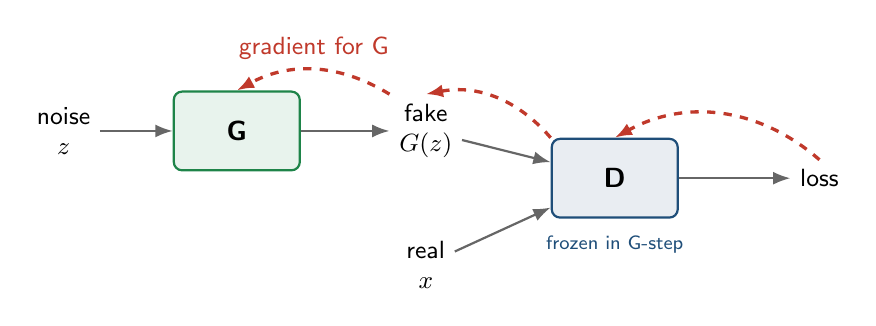
\begin{tikzpicture}[
    net/.style={draw, thick, rounded corners=3pt, minimum width=1.6cm,
      minimum height=1cm, font=\sffamily\bfseries},
    dat/.style={font=\sffamily\small, align=center},
    fwd/.style={-{Latex[length=2.2mm]}, thick, black!60},
    bwd/.style={-{Latex[length=2.2mm]}, very thick, wrongc, dashed}]
  \node[dat] (z) at (0,0) {noise\\$z$};
  \node[net, draw=rightc, fill=rightc!10] (G) at (2.2,0) {G};
  \node[dat] (xf) at (4.6,0) {fake\\$G(z)$};
  \node[dat] (xr) at (4.6,-1.7) {real\\$x$};
  \node[net, draw=accent, fill=accent!10] (D) at (7,-0.6) {D};
  \node[dat] (L) at (9.6,-0.6) {loss};
  \node[font=\sffamily\scriptsize, text=accent] at (7,-1.45) {frozen in G-step};
  \draw[fwd] (z) -- (G);
  \draw[fwd] (G) -- (xf);
  \draw[fwd] (xf) -- (D);
  \draw[fwd] (xr) -- (D);
  \draw[fwd] (D) -- (L);
  \draw[bwd] (L.north) to[bend right=35] (D.north);
  \draw[bwd] (D.north west) to[bend right=30] (xf.north);
  \draw[bwd] (xf.north west) to[bend right=30]
    node[above, font=\sffamily\small] {gradient for G} (G.north);
\end{tikzpicture}}{The generator's loss is measured at the discriminator's
output. Its gradient must travel back \emph{through} D (with D's weights frozen)
to reach G. Without D there is no training signal for G.}

\begin{center}\small
\begin{tabularx}{\linewidth}{@{}>{\raggedright\arraybackslash}p{5.3cm}c X@{}}
  \toprule
  Statement & Answer & Reason \\
  \midrule
  Generator learns the (empirical) probability function & \bad{} False & G is
    an \emph{implicit} model: a sampler $z\mapsto x$, not a density you can evaluate \\
  All GANs require labeled data $(x,y)$ & \bad{} False & the basic GAN needs only
    real images; real/fake labels are generated automatically \\
  CycleGAN trains two generators and two discriminators & \ok{} True &
    $G\colon X\to Y$, $F\colon Y\to X$, plus $D_X$, $D_Y$ and the cycle loss \\
  Generator backprop is independent of the discriminator & \bad{} False &
    the gradient flows through D (figure above) \\
  \bottomrule
\end{tabularx}
\end{center}

\begin{hook}
Explicit density estimators: MLE, Parzen windows, (restricted) Boltzmann machines.
A GAN only \emph{samples}. Check whether the question asks for ``estimating a
distribution'' or ``generating samples'' (Q28).
\end{hook}

% ================================================================= checklist
\topic{Checklist Before Submitting}{}\label{sec:check}

\begin{center}
\begin{tabularx}{\linewidth}{@{}c>{\raggedright\arraybackslash}X@{}}
  $\square$ & Multi-select: every option judged on its own? \\
  $\square$ & ``always'', ``only'', ``necessarily'' checked? \\
  $\square$ & Invariance/equivariance, inputs/gradients, width/depth not swapped? \\
  $\square$ & Hough: $\rho = x\cos\theta + y\sin\theta$ computed for every option? \\
  $\square$ & Conv parameters: $K\cdot K\cdot C_\text{in}\cdot C_\text{out}$, spatial size irrelevant? \\
  $\square$ & R-table: orientation range ($\bmod 180^\circ$ or $\bmod 360^\circ$) checked? \\
  $\square$ & Histograms: axis orientation fixed with the unambiguous patch? \\
  $\square$ & Saliency: entropy \emph{peak over scale}, not maximum entropy? \\
  $\square$ & Bayes: evidence $=$ sum over \emph{all} hypotheses, round only at the end? \\
  $\square$ & Discriminant: likelihood \emph{and} prior (or the posterior)? \\
  $\square$ & BPTT: unroll, one factor per time step, ignore distractor values? \\
\end{tabularx}
\end{center}

\end{document}
